\documentclass[11pt]{article}
\usepackage{graphicx}
\usepackage[margin=2.5cm]{geometry}
\usepackage{tikz}
\usepackage{indentfirst}
\usepackage{tabularx}
\usepackage{listingsutf8}
\usepackage{color}
\usepackage{hyperref}
\usepackage{float}
\usepackage[portuguese]{babel}

\graphicspath{{./images/}}

\def\checkmark{\tikz\fill[scale=0.4](0,.35) -- (.25,0) -- (1,.7) -- (.25,.15) -- cycle;} 
\setlength{\parskip}{0.5em}

\renewcommand{\lstlistingname}{Código}
\renewcommand{\lstlistlistingname}{Pedaços de Código}

\definecolor{dkgreen}{rgb}{0,0.6,0}
\definecolor{gray}{rgb}{0.5,0.5,0.5}
\definecolor{mauve}{rgb}{0.58,0,0.82}

\hypersetup{
	colorlinks=false,
	linktoc=all,
	hidelinks,
}

\lstset{
	belowcaptionskip=1\baselineskip,
	captionpos=b,
	frame=tb,
	language=C,
	aboveskip=3mm,
	belowskip=3mm,
	showstringspaces=false,
	columns=flexible,
	basicstyle={\small\ttfamily},
	numbers=none,
	numberstyle=\tiny\color{gray},
	keywordstyle=\color{blue},
	commentstyle=\color{dkgreen},
	stringstyle=\color{mauve},
	breaklines=true,
	breakatwhitespace=true,
	tabsize=3,
	inputencoding=utf8,
	extendedchars=true,
	literate={á}{{\'a}}1 {ã}{{\~a}}1 {à}{{\`a} }1 {Ã}{{\~A}}1 {ó}{{\'o}}1 {Ó}{{\'O}}1 {Í}{{\'I}}1 {í}{{\'i}}1 {é}{{\'e}}1 {ç}{{\c{c}}}1 {Ç}{{\c{C}}}1 {ú}{{\'u}}1 {õ}{{\~o}}1
}

\begin{document}
	\begin{titlepage}
    	\begin{center}
    		
\includegraphics[width=0.6\textwidth]{logo-isec}
    		
    		\vspace*{\fill}
    		
    		\Huge
    		\textbf{Sistemas Operativos II}
    		
    		\huge
    		Sistema de Gestão do Espaço Aéreo
    		
    		\vspace{0.5cm}
    		\LARGE
    		2020 - 2021
    		
    		\vspace{1.5cm}
    		
    		\textbf{TheForgotten\\BrunoTeixeira1996}
    		
    		\vfill
    		\vspace*{\fill}
    		
    		\normalsize
    		Licenciatura de Engenharia Informática \\
    		13 de junho de 2021		
    	\end{center}
    \end{titlepage}
	
	\tableofcontents
	\pagebreak
	
	\large
	\section{Introdução}
	\normalsize
	
	O trabalho prático consiste na implementação de vários programas que, no seu conjunto, simulam um sistema de gestão de aeroportos, espaço aéreo, passageiros e aviões que nele circulam.
	
	O trabalho prático foi concretizado em linguagem C usando a API do Windows chamada de Win32. Para esta segunda meta foi criada uma GUI para o \textbf{Control}, mantendo o paradigma de consola para as restante aplicações.
	
	\begin{figure}[h]
		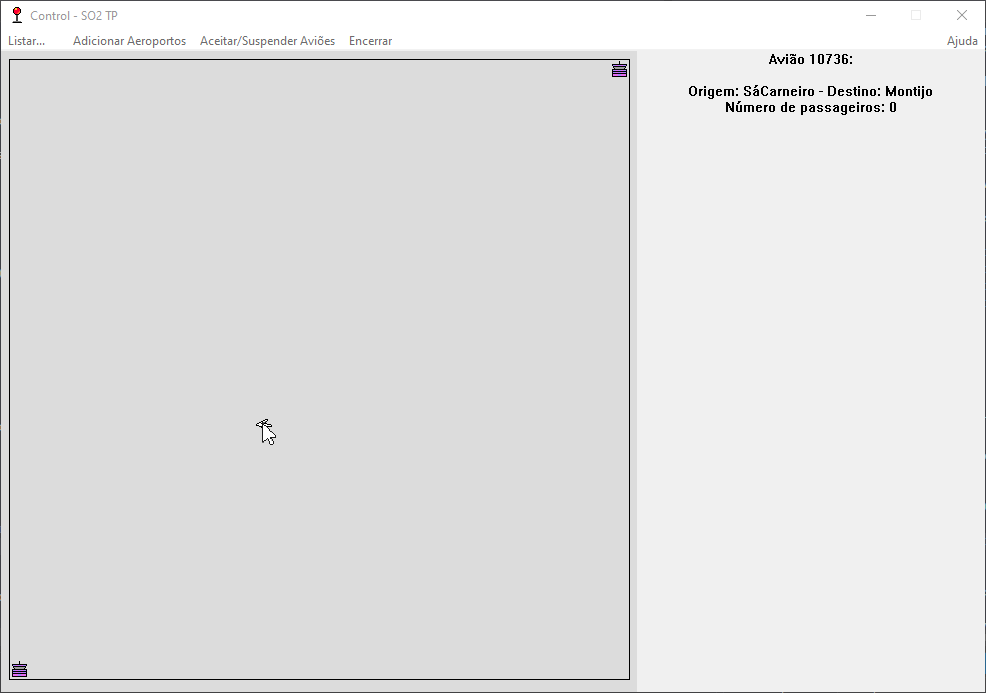
\includegraphics[width=0.95\textwidth,height=0.88\textheight,keepaspectratio]{control-airplane}
		\centering
		\caption{Control - Hover num Avião}
		\label{fig:control-airplane}
	\end{figure}
	
	\begin{figure}[H]
		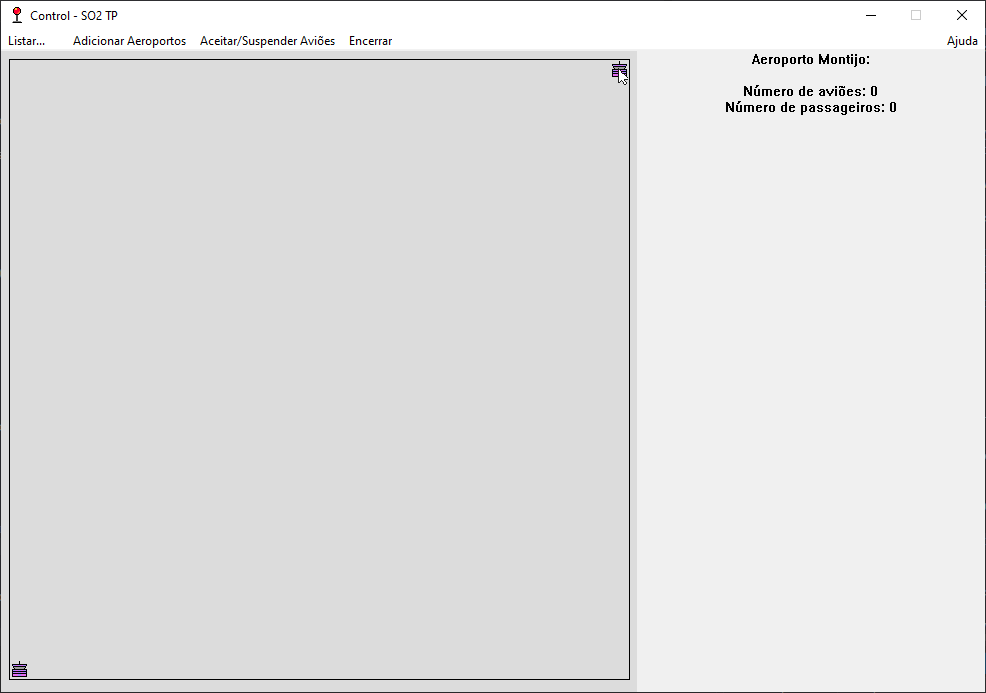
\includegraphics[width=0.95\textwidth,height=0.88\textheight,keepaspectratio]{control-airport}
		\centering
		\caption{Control - Clique num Aeroporto}
		\label{fig:control-airport}
	\end{figure}
    
    
	\large
	\section{Correções Feitas Após a Primeira Meta}
	\normalsize
	
	Agora toda a comunicação do avião com o Control é única e exclusivamente feita por buffer circular, ao contrário do que era feito na 1ª meta.
	
	Os aeroportos já não se encontram no Registry. Em vez disso, existe um bloco de memória partilhada onde os aviões acedem aos aeroportos que existem.
	
	Agora o avião assinala um evento para escrever a sua estrutura atualizada no buffer circular quando se move, ao contrário do que fazia antes que escrevia diretamente na memória partilhada das coordenadas.
	
	A memória partilhada que era usada para escrever aviões e ver que coordenadas estavam ou não ocupadas é agora exclusivamente para as coordenadas, os aviões apenas leêm o bloco de memória, não lhe fazendo alterações. Este bloco é atualizado apenas pelo Control, uma vez que o Control é que contém essas coordenadas localmente.
    
    
	\large
	\section{Arquitetura Geral}
	\normalsize
	
	A aplicação \textbf{Control} é a responsável por gerir todo o funcionamento do espaço aéreo. Sem esta, nem os aviões nem os passageiros conseguem funcionar. Deste modo, esta deve ser sempre aberta antes dos outros.
	
	Depois é só inicializar quantos aviões desejar, estes comunicarão com o \textbf{Control} por buffer circular usando o paradigma produtor/consumidor, sendo o avião considerado o produtor e o controlador o consumidor.
	
	O avião irá avisar o \textbf{Control} momentaneamente de que este se encontra ligado e a funcionar normalmente, usando uma thread para isso.
	
	Depois o processo de verificação de posições ocupadas por parte dos aviões, é feita também com memória partilhada, uma vez que o controlador vai atualizando a memória partilhada com as coordenadas ocupadas, o avião gera umas novas coordenadas com a \textbf{DLL} disponibilizada e depois vai verificar nessa memória partilhada se essas coordenadas estão ou não livres, caso não estejam o mesmo volta a gerar outras coordenadas sempre usando a \textbf{DLL} para esse efeito.
	
	Os passageiros comunicam com o \textbf{Control} usando named pipes. Os passageiros nunca comunicam diretamente com os aviões, nem vice-versa. Podemos abrir quantos passageiros desejarmos, indicando por argumento o nome, onde está, para onde quer ir e, opcionalmente, quanto tempo (em segundos) fica à espera para embarcar.
	
	
	\large
	\section{Mecanismos de Sincronização}
	\normalsize
	
	Para garantir que apenas existe uma instância da aplicação \textbf{Control} é usado um semáforo com nome. Para gerir dados partilhados entre threads do mesmo processo são usadas secções críticas. No entanto para gerir dados entre processos diferentes usamos um mutex com nome.
	
	O \textbf{Control} garante também que apenas são permitidos aviões consoante o número máximo definido no início da execução. Este controlo é feito usando um semáforo que é criado no início da execução do \textbf{Control}, semáforo este que apenas tem lugar igual ao número máximo de aviões permitidos.
	
	O mecanismo de \textbf{ping} do avião em relação ao \textbf{Control} funciona com eventos com nome. É criado um evento com um nome genérico baseado no ID de processo do avião, e depois é aberto no lado do \textbf{Control}. Este fica 3 segundos à espera do evento ser assinalado e, no caso de não ser assinalado, deixa de dar atenção ao avião e assume que deixou de existir.
	
	No paradigma de produtor/consumidor, uma vez que existem \textbf{N} produtores e apenas um consumidor, usamos dois semáforos, um de leitura e outro de escrita, usamos também algumas secções criticas dentro dos processos e usamos um mutex apenas para o produtor, de modo a garantirmos um correto funcionamento do paradigma.
	
	Dentro do \textbf{Control}, de modo a informar as threads de passageiro que há um avião há procura de passageiros para embarcar, são usados eventos e, de modo a diminuir o tráfego no acesso à informação sobre os aviões, são usados eventos com nomes genéricos. A cada instância que se liga ao \textbf{named pipe} é atribuida uma thread que lida com a leitura e escrita no mesmo.
	
	
	\large
	\section{Uso da DLL}
	\normalsize
	
	Na nossa implementação, decidimos usar a \textbf{DLL} de forma explícita por acharmos que traz mais vantagens em relação à implícita.
	
	O código não é muito mais difícil na explícita e, para além disso, com este tipo de implementação é muito mais fácil fazer mudanças na \textbf{DLL}. Também nos agradou o facto de não ser preciso fazer alterações nas definições de projeto no Visual Studio.
	
	\large
	\section{Estruturas de Dados}
	\subsection{Struct COORDINATES}
	\normalsize
	
	\begin{lstlisting}[caption=Struct COORDINATES]
	    struct COORDINATES_STRUCT{
	        int x, y;
	    };
	\end{lstlisting}
	
	Estrutura responsável pelas coordenadas.
	
	
	\large
	\subsection{Struct SHARED\_COORDINATES}
	\normalsize

	\begin{lstlisting}[caption=Struct SHARED\_COORDINATES]
		struct SHARED_COORDINATES_STRUCT {
        	int x, y;
        	unsigned int maxAirplanes;
        };
	\end{lstlisting}

	Estrutura utilizada para o uso da memória partilhada para a verificação das coordenadas.
	
	
    \large
	\subsection{Struct AIRPLANE}
	\normalsize

	\begin{lstlisting}[caption=Struct AIRPLANE]
		struct AIRPLANE_STRUCT {
			   DWORD id;
	           unsigned int capacity, velocity;
	           coordinatesStruct currentCoordinates; // coordenadas atuais
	           coordinatesStruct destinationCoordinates; // coordenadas do destino
	           TCHAR destAirport[STR_SIZE], srcAirport[STR_SIZE];
	           BOOL stopped; // está parado ?
		};
	\end{lstlisting}

	Esta é a estrutura associada aos aviões. Cada avião vai estar associado a uma estrutura destas.
	
	
	\large
	\subsection{Struct AIRPORT}
	\normalsize

	\begin{lstlisting}[caption=Struct AIRPORT]
		struct AIRPLANE_STRUCT {
		        TCHAR name[STR_SIZE];

            	coordinatesStruct coordinates;
            
            	unsigned int maxAirports;
            
            	unsigned int currentPassengers;
		};
	\end{lstlisting}

	Esta é a estrutura associada aos aeroportos. Cada aeroporto vai estar associado a uma estrutura destas.
	
	
	
	\large
	\subsection{Struct PASSENGER}
	\normalsize

	\begin{lstlisting}[caption=Struct PASSENGER]
		struct AIRPLANE_STRUCT {
		        TCHAR name[STR_SIZE];
            	DWORD id, airplaneId;
            
            	TCHAR destAirport[STR_SIZE], srcAirport[STR_SIZE];
            
            	unsigned int waitToBoard;
            
            	BOOL stopped;
		};
	\end{lstlisting}

	Esta é a estrutura associada aos aeroportos. Cada aeroporto vai estar associado a uma estrutura destas.
	
	
	\large
	\subsection{Struct SHAREDMEM}
	\normalsize
	
	\begin{lstlisting}[caption=Struct SHAREDMEM\_STRUCT]
        struct SHAREDMEM_STRUCT {
        	int nProducers;
        	int writeIndex; // Próxima posição de escrita
        	int readIndex; // Próxima posição de leitura
        
        	airplane buffer[CIRCULAR_BUFFER_SIZE]; // Buffer circular em si (array de estruturas)
        };
	\end{lstlisting}
	
	Estrutura utilizada para o uso da memória partilhada usando o paradigma produtor/consumidor.
	
	
	\large
	\section{Controlador Aéreo}
	\subsection{Funcionalidades principais}
	\subsubsection{Controlo da informação de aeroportos e aviões}
	\normalsize
	
    Toda a informação relativamente aos aeroportos, aviões e passageiros está guardada localmente no \textbf{Control} para que fique mais fácil manipular todas as estruturas de dados.
    O \textbf{Control} guarda também um array de handles usado na thread de avisos dos aviões, assim como um array de estruturas dos \textbf{Pings}.
    
    Na nossa interface representamos o mapa em escala, ou seja, representamos o campo 1000x1000 num espaço de 600x600. Esta escala pode facilmente ser alterada.
	
	
	\large
	\subsubsection{Criação de aeroportos}
	\normalsize
	
	Usando o botão "Adicionar Aeroportos" do menu superior podemos adicionar aeroportos. Este botão irá abrir uma \textbf{dialog box} onde podemos inserir todos os dados necessários à criação do mesmo. A informação recolhida é então tratada e passada para dentro da função \textit{caeroporto}, que irá tratar de adicionar o aeroporto ao array.
	
	
	\large
	\subsubsection{Atualização das posições dos aviões}
	\normalsize
	
	O \textbf{Control} tem uma thread responsável por interagir com a memória partilhada (\textbf{coordinatesThread}), memória esta que é usada pelo avião para verificar a ocupação de posições.
	
	Inicialmente o \textbf{Control} preenche a memória partilhada com um array de estruturas do tipo \textbf{SHARED\_COORDINATES}, tendo estas estruturas a informação do número de aviões existentes e as coordenadas ocupadas.
	
	Depois, em curtos intervalos de tempos, vai atualizando este espaço de memória, mantendo sempre neste espaço apenas as coordenadas ocupadas. O número de aviões existentes também vai sendo atualizado.
	
	
	\large
	\section{Aviões}
	\normalsize
	
	O programa \textbf{Airplanes} representa cada instância de um avião distinto. Este programa é lançado pelo utilizador e faz várias viagens. 
	
	
	\large
	\subsection{Funcionalidades principais}
	\subsubsection{Lançamento}
	\normalsize
	
	No início da execução, é pedido ao utilizador a lotação, a velocidade em posições por segundo e o aeroporto inicial onde se encontra.
	
	Depois de serem validados todos os parâmetros introduzidos pelo utilizador, o avião vai ao buffer circular que está em memória partilhada com o \textbf{Control} e escreve lá a sua estrutura, como uma espécie de inscrição.
	
	
	\large
	\subsubsection{Movimentação no espaço aéreo}
	\normalsize
	
	O avião antes de iniciar a movimentação gera umas coordenadas usando a \textbf{DLL} e logo de seguida vê se o \textbf{Mutex} partilhado entre ele e o \textbf{Control} está livre, caso esteja significa que a memória partilhada ja contém as coordenadas ocupadas atualizadas. De seguida o avião acede à memória partilhada e verifica se as coordenadas geradas pela \textbf{DLL} são ou não válidas, caso sejam, o mesmo aciona um evento que irá pedir a uma thread interna para escrever a sua struct de novo no buffer circular e avança uma posição, caso não sejam o avião volta a chamar a \textbf{DLL} até encontrar umas coordenadas válidas. Se chegar ao fim a \textbf{DLL} retorna 0, sendo assim o mesmo aciona o evento mencionado anteriormente e muda o seu estado \textbf{hasArrivedAtDestination} para \textbf{TRUE}.
	
	Uma vez que a \textbf{DLL} fornece coordenadas seguidas (1,1 ou 2,2, ...) tivemos de implementar uma solução para isto. A solução encontrada foi, no processo de chamada à \textbf{DLL}, as coordenadas do aeroporto de destino foram alteradas de maneira aleatória, somando um valor entre 0 e 1000 às mesmas (valores corrigidos na seguinte iteração), forçando o avião a ir por um caminho alternativo nunca entrando em colisão contra outro avião.
	
	
	\large
	\section{Passageiros}
	\normalsize

    O programa \textbf{Passengers} representa cada instância de um passageiro distinto. Este programa é lançado pelo utilizador e faz apenas uma viagem. 
    
    
    \large
	\subsection{Funcionalidades principais}
	\subsubsection{Lançamento}
	\normalsize
	
	Ao iniciar o programa, deve ser indicado por argumento o nome do passageiro, donde parte, para onde quer ir e quanto tempo fica à espera para embarcar, sendo este último opcional.
	
	Após isto, ele apenas serve para imprimir informação, não voltando a receber mais dados do utilizador.
    

	\large
	\section{Manual de Utilização}
	\subsection{Control}
	\normalsize
	
	Para receber ajuda quanto à utilização desta aplicação basta usar a opção "Ajuda" no menu.
	
	
	\large
	\subsection{Airplanes}
	\normalsize
	
	\begin{tabularx}{\textwidth}{|l|X|X|}
	    \hline
	    \textbf{Comando} & \textbf{Modo de uso} & \textbf{Descrição} \\
	    \hline
	    destino & destino \textless{nome\_aeroporto}\textgreater & Define o destino do avião \\
	    \hline
	    embarcar & embarcar & Avisa o Control que pretende que passageiros embarquem \\
	    \hline
	    inicia & inicia & Inicia a viagem \\
	    \hline
	    terminar & terminar & Desliga o programa \\
	    \hline
	\end{tabularx}
	
	
	\large
	\subsection{Passageiros}
	\normalsize
	
	Esta aplicação não aceita qualquer tipo de interação do utilizador depois de estar aberta. Para isso, deve ser aberta com argumentos, usando o template \textit{app.exe \textless{nome}\textgreater \textless{aeroporto origem}\textgreater \textless{aeroporto destino}\textgreater \textless{tempo espera (opcional)}\textgreater}, onde \textit{nome} é o nome do passageiro em particular, \textit{aeroporto origem} é o aeroporto onde este inicialmente se encontra, \textit{aeroporto destino} o aeroporto para onde este se pretende dirigir e o \textit{tempo espera} o tempo máximo que este fica a aguardar por embarcar, podendo não ser mencionado ou ser dado o valor '0' e, se assim for, fica à espera infinitamente.
	
	
	\large
	\subsection{Reg}
	\normalsize

    Reg é uma pequena aplicação feita com o intuito de facilitar a criação das chaves no \textbf{registry} do Windows.
    
    Esta começa por perguntar o que pretendemos que seja o número máximo de aviões e o que pretendemos que seja o número máximo de aeroportos. Em seguida cria as chaves e os atributos valor no \textbf{registry}, tendo a chave o path "HKEY\_CURRENT\_USER\textbackslash{SOFTWARE}\textbackslash{SO2-TP}\textbackslash{MaximumValues}" e sendo os atributos valor "MaxAirplanes" e "MaxAirports".
	
	
	\large
	\section{Tabela de Funcionalidades Implementadas}
	\normalsize
    \begin{tabularx}{\textwidth}{|c|X|c|}
        \hline
        \textbf{ID} & \textbf{Descrição da Funcionalidade / Requisito} & \textbf{Estado} \\
        \hline
        0 & Interface Gráfica para Control & Implementada \\ 
        \hline
        1 & Mouseover do Rato em Cima de um Avião em Voo Mostra Informação Adicional & Implementada \\
        \hline
        2 & Click do rato em cima de um aeroporto mostra informação adicional  & Implementada \\
        \hline
        3 & Menu e Dialogbox na Interface Gráfica & Implementada \\
        \hline
        4 & Visualização do Espaço Aéreo & Implementada \\ 
        \hline
        5 & Uso de AlphaBlend (não requisito) & Implementada \\ 
        \hline
        6 & Criação de BMPs 16x16 para aeroporto, avião e ícone do Control & Implementada \\ 
        \hline
        7 & Buffer Circular (Comunicação Control \textless{-} Aviões) & Implementada \\ 
        \hline
        8 & Movimentação dos Aviões (com recurso à DLL) & Implementada \\ 
        \hline
        9 & Ping dos Aviões ao Control & Implementada \\
        \hline
        10 & Não Colisão dos Aviões & Implementada \\ 
        \hline
        11 & Passageiros & Implementada \\ 
        \hline
        12 & Comunicação Control \textless{-}\textgreater Passageiros com Named Pipes & Implementada \\ 
        \hline
        13 & Tirar Valores Máximos do Registry & Implementada \\ 
        \hline
        14 & Garantir que Existe Apenas 1 Control & Implementada \\ 
        \hline
        15 & Aeroportos (possuir nome único e serem únicos num raio (quadrado) de 10) & Implementada \\ 
        \hline
    \end{tabularx}
    
    Temos confiança que implementamos todo o que era requisitado e ainda mais algumas coisas que achamos que davam \textit{flavor} ao produto final.
    
	\large
	\section{Conclusão}
	\normalsize
	
	Ao longo deste trabalho, deparámo-nos e fomos resolvendo vários desafios que não esperávamos ter, tratando-se de uma excelente oportunidade para consolidação de matéria das aulas teóricas e práticas de Sistemas Operativos 2. Este permitiu-nos colocar em prática conceitos importantes sobre a arquitetura, criação e desenvolvimento de programas para sistemas NT, dando-nos uma visão para os vários detalhes dessas atividades.
	
	\pagebreak
	
	
	\large
	\section{Anexos}
	\normalsize
	
	\listoffigures
	\lstlistoflistings
\end{document}